
\documentclass[9pt]{beamer}
%\makeatletter
%\def\beamer@calltheme#1#2#3{%
%	\def\beamer@themelist{#2}
%	\@for\beamer@themename:=\beamer@themelist\do
%	{\usepackage[{#1}]{\beamer@themelocation/#3\beamer@themename}}}
%
%\def\usefolder#1{
%	\def\beamer@themelocation{#1}
%}
%\def\beamer@themelocation{}

%\usefolder{../config}

\usetheme[
block=fill,
titleformat=regular,
progressbar=frametitle
]{metropolis}
%\metroset[everytitleformat=regular] % regular, lowercase, uppercase ]
%\metroset[inner/block=fill]

%\setbeameroption{show notes} 
\usepackage{booktabs}
\usepackage[scale=2]{ccicons}

\usepackage{pgfplots}
\usepgfplotslibrary{dateplot}


%\ Hrvatski znakovi
\usepackage[utf8]{inputenc}
\usepackage[T1]{fontenc}
\usepackage[croatian]{babel}
\usepackage{todonotes}
\usepackage{amsmath}
\usepackage{amsfonts}
\selectlanguage{croatian} % american ngerman
\usepackage{todonotes}

% Koristenje Latin modern fonta
% Bez toga na nekim racunalima baca
% err: Font <taj i taj> at <mala velicina, npr4.0pt> not loadable: Metric (TFM) file not found. \end{frame}
\usepackage{lmodern}


\definecolor{RoyalBlue}{cmyk}{1, 0.50, 0, 0}
%\usepackage{natbib}
%\usepackage{bibentry}
\usepackage{scrextend}
\usepackage{hyperref}
%\usepackage[pdfa=true]{hyperref}
\hypersetup{%
    %draft, % = no hyperlinking at all (useful in b/w printouts)
    %colorlinks=true, 
    linktocpage=true, pdfstartpage=3, pdfstartview=FitV,%
    % uncomment the following line if you want to have black links (e.g., for printing)
    %colorlinks=false, linktocpage=false, pdfborder={0 0 0}, pdfstartpage=3, pdfstartview=FitV,% 
    breaklinks=true, pdfpagemode=UseNone, pageanchor=true, pdfpagemode=UseOutlines,%
    plainpages=false, bookmarksnumbered, bookmarksopen=true, bookmarksopenlevel=1,%
    hypertexnames=true, pdfhighlight=/O,%nesting=true,%frenchlinks,%
    %urlcolor=webbrown, linkcolor=RoyalBlue, citecolor=webgreen, %pagecolor=RoyalBlue,%
    %urlcolor=Blue, linkcolor=Blue, citecolor=Red, %pagecolor=Black,%
    %pdftitle={\myTitle},%
    %pdfauthor={\textcopyright\ \myName, \myUni, \myFaculty},%
    pdfsubject={},%
    pdfkeywords={},%
    pdfcreator={pdfLaTeX},%
    pdfproducer={LaTeX with hyperref and classicthesis}, %
    unicode = true 
} 

%\usepackage[pdftex]{graphicx}
% declare the path(s) where your graphic files are
\graphicspath{{./}{./figures/}}


\newcommand{\executeiffilenewer}[3]{%
	\ifnum\pdfstrcmp{\pdffilemoddate{#1}}%
	{\pdffilemoddate{#2}}>0%
	{\immediate\write18{#3}}\fi%
}
\newcommand{\includesvg}[1]{%
	\executeiffilenewer{#1.svg}{#1.pdf}%
	{inkscape -z -C --file=#1.svg %
		--export-pdf=#1.pdf --export-latex}%
	\input{#1.pdf_tex}%
}


% http://tex.stackexchange.com/questions/83882/how-to-highlight-python-syntax-in-latex-listings-lstinputlistings-command

\usepackage{listings}
\usepackage{color}
\usepackage[semibold]{sourcecodepro}

% Default fixed font does not support bold face
\DeclareFixedFont{\ttb}{T1}{txtt}{bx}{n}{12} % for bold
\DeclareFixedFont{\ttm}{T1}{txtt}{m}{n}{12}  % for normal
% Custom colors
\definecolor{deepblue}{rgb}{0,0,0.5}
\definecolor{deepred}{rgb}{0.6,0,0}
\definecolor{deepgreen}{rgb}{0,0.5,0}


% Python style for highlighting
\newcommand\pythonstyle{\lstset{
		language=Python,
		basicstyle=\small\ttfamily,
		otherkeywords={self},             % Add keywords here
		keywordstyle=\small\ttfamily\color{deepblue},
		emph={MyClass,__init__},          % Custom highlighting
		emphstyle=\small\ttfamily\color{deepred},    % Custom highlighting style
		stringstyle=\color{deepgreen},
		frame=tb,                         % Any extra options here
		showstringspaces=false            % 
	}}
	
	
	% Python environment
	\lstnewenvironment{python}[1][]
	{
		\pythonstyle
		\lstset{#1}
	}
	{}
	
	% Python for external files
	\newcommand\pythonexternal[2][]{{
			\pythonstyle
			\lstinputlisting[#1]{#2}}}
	
	% Python for inline
	\newcommand\pythoninline[1]{{\pythonstyle\lstinline!#1!}}

% \includeonlyframes{current}

%\documentclass[ucs]{beamer}
%\usetheme[menuwidth={0.3\paperwidth}]{erlangen}
%\setbeamercovered{transparent=20} 

\usepackage{amsmath,amsfonts,amsthm,amssymb}
\usepackage{setspace}
\usepackage{Tabbing}
\usepackage{fancyhdr}
\usepackage{lastpage}
\usepackage{extramarks}
\usepackage{chngpage}
\usepackage{soul,color}
\usepackage{graphicx,float,wrapfig}
\usepackage{xcolor}
\usepackage[normalem]{ulem}
\usepackage{mathtools}

\definecolor{erlangenlyellow}{RGB}{123, 25, 121}
%\usepackage[utf8x]{inputenc}
%\usepackage{default}
%\usepackage[T1]{fontenc}

\usepackage{verbatim}
\usepackage{listings}


\usepackage{subcaption}
\usepackage{lmodern}

\title{Projecting Projection Project}

\subtitle{ This is the way to build our castle in the sky}
\institute{Računalna grafika}


\begin{document}
\begin{frame}
 \titlepage
\end{frame}

%\begin{frame}{Sadržaj}
%  \tableofcontents
%  % You might wish to add the option [pausesections]
%\end{frame}
\section{Rotacija oko proizvoljne osi}
\begin{frame}{Proizvoljna os}
	Os možemo zadati točkom $P$ i vektorom $V$.
	\begin{center}
		\includegraphics[width=5cm]{./slike/p04_01.png}
	\end{center}
	Cilj je \textit{poravnati} vektor $\vec{v}$ sa $z$ osi.
\end{frame}

\begin{frame}{Translacija u ishodište}
	\begin{center}
		\includegraphics[width=5cm]{./slike/p04_01a.png}
	\end{center}
	\begin{align*}
	\mathbf{T}_{-P} = \left[ \begin{array}{cccc}
	1 & 0 & 0 & 0 \\
	0 & 1 & 0 & 0 \\
	0 & 0 & 1 & 0 \\
	-x_P & -y_P & -z_P & 1 
	\end{array} \right]
	\end{align*}
\end{frame}


\begin{frame}{Rotacija oko $y$ osi}
	\begin{columns}
		\begin{column}{0.48\textwidth}
			\begin{center}
				\includegraphics[width=4cm]{./slike/p04_02.png}
			\end{center}
		\end{column}
		\begin{column}{0.48\textwidth}
			\begin{align*}
			\theta= \arctan \frac{x_v}{z_v}
			\end{align*}
			Treba rotirati za $-\theta$.
			\begin{align*}
			\mathbf{R}_{y_{-\theta}} = \left[ \begin{array}{cccc}
			\cos (-\theta) & 0 & \sin (-\theta) & 0 \\
			0 & 1 & 0 & 0 \\
			-\sin(-\theta) & 0 & \cos(-\theta) & 0 \\
			0 & 0 & 0 & 1 
			\end{array} \right]
			\end{align*}
		\end{column}
	\end{columns}
\end{frame}

\begin{frame}{Rotacija oko $x$ osi}
	\begin{columns}
		\begin{column}{0.48\textwidth}
			\begin{center}
				\includegraphics[width=4cm]{./slike/p04_03.png}
			\end{center}
		\end{column}
		\begin{column}{0.48\textwidth}
			\begin{align*}
			\phi= \arctan \frac{y_v}{\sqrt{x_v^2 + z_v^2}}
			\end{align*}
			Treba rotirati za $\phi$.
			\begin{align*}
			\mathbf{R}_{x_{\phi}} =  \left[ \begin{array}{cccc}
			1 & 0 & 0 & 0 \\
			0 & \cos\phi & \sin\phi & 0 \\
			0 & -\sin\phi & \cos\phi & 0 \\
			0 & 0 & 0 & 1 
			\end{array} \right]
			\end{align*}
		\end{column}
	\end{columns}
\end{frame}

\begin{frame}{Rotacija oko osi za kut $\alpha$:}
	\begin{columns}
		\begin{column}{0.48\textwidth}
			\begin{center}
				\includegraphics[width=4cm]{./slike/p04_04.png}
			\end{center}
		\end{column}
		\begin{column}{0.48\textwidth}
			Transformacije do sada:
			\begin{align*}
			\mathbf{T}_{-P}\mathbf{R}_{y_{-\theta}}\mathbf{R}_{x_{\phi}}
			\end{align*}
			Sada možemo odraditi rotaciju za kut $\alpha$:
			\begin{align*}
			\mathbf{R}_{\alpha} =  \left[ \begin{array}{cccc}
			\cos\theta & \sin\theta & 0 & 0 \\
			-\sin\theta & \cos\theta & 0 & 0 \\
			0 & 0 & 1 & 0 \\
			0 & 0 & 0 & 1 
			\end{array} \right]
			\end{align*}
		\end{column}
	\end{columns}
\end{frame}



\begin{frame}{Tek sada ćemo biti gotovi}
	\begin{columns}
		\begin{column}{0.48\textwidth}
			\begin{block}{Transformacije do sada:}
				\begin{align*}
				\mathbf{T}_{-P}\mathbf{R}_{y_{-\theta}}\mathbf{R}_{x_{\phi}}\mathbf{R}_{\alpha}
				\end{align*}
			\end{block}
		\end{column}
		\begin{column}{0.48\textwidth}
			Transformacije do sada:
			Još se moramo vratiti:
			\begin{itemize}
				\item Rotirati oko osi $x$ za $-\phi$
				\item Rotirati oko osi $y$ za $\theta$
				\item Translacija natrag za $P$
			\end{itemize}
		\end{column}
	\end{columns}
	\begin{block}{Krajnji izraz:}
		\begin{align*}
		\mathbf{R}_{osPV} = \mathbf{T}_{-P}\mathbf{R}_{y_{-\theta}}\mathbf{R}_{x_{\phi}}\mathbf{R}_{\alpha}\mathbf{R}_{x_{-\phi}}\mathbf{R}_{y_{\theta}}\mathbf{T}_{P}
		\end{align*}
		Dakle, ako želimo rotirati točku oko osi za kut $\alpha$:
		\begin{align*}
		\left[ \begin{array}{cccc} x' & y' & z' & 1 \end{array} \right] = \left[ \begin{array}{cccc}
		x & y & z & 1 \end{array} \right] \mathbf{R}_{osPV}
		\end{align*}
	\end{block}
\end{frame}

\section{4d projektivni prostor}
\begin{frame}{Uvod}
	\begin{align*}
	\left[ \begin{array}{cccc}
	x & y & z & 1 \end{array} \right] 
	\left[ \begin{array}{cccc}
	&  &  & 0 \\
	&  &  & 0 \\
	&  &  & 0 \\
	&  &  & 1 
	\end{array} \right] \left[ \begin{array}{cccc} x' & y' & z' & 1 \end{array} \right] 
	\end{align*}
	ili:
	\begin{align*}
	\left[ \begin{array}{cccc}
	x & y & z & 1 \end{array} \right] 
	\left[ \begin{array}{cccc}
	&  &  & a \\
	&  &  & b \\
	&  &  & c \\
	&  &  & d 
	\end{array} \right] \left[ \begin{array}{cccc} x' & y' & z' & w \end{array} \right] 
	\end{align*}
\end{frame}

\begin{frame}{Projekcija na $w=1$}
	\begin{center}
		\includegraphics[width=5cm]{./slike/p04_05.png}
	\end{center}
	Vrijede relacije:
	$\frac{x'}{1} = \frac{x}{w}$, $\frac{y'}{1} = \frac{y}{w}$, $\frac{z'}{1} = \frac{z}{w}$\\
	$x' = \frac{x}{w}$, $y' = \frac{y}{w}$, $z' = \frac{z}{w}$\\
	Ima li smisla $w=0$? Pravac koji prolazi kroz ishodište i točku za $w=0$ - nema sjecišta sa $w=1$ \\
	Ima li smisla $w < 0$? - Crvena linija
\end{frame}
\section{Transformacije pogleda}
\begin{frame}{View - Camera space}
	Nakon što se odabere mjesto i smjer gledanja:
	
	\begin{itemize}
		\item Prostor se kreira projekcijom, odnosno projekcijom scene ispred kamere.
		\item Kamera je \textit{holografski} projektor koji projicira scenu na monitor.
		\item Oblik prostora može biti:
		\begin{itemize}
			\item kvadar (\textbf{paralelna projekcija})
			\item odsječak piramide(\textbf{perspektivna projekcija})  
		\end{itemize}
		\item Volumen perspektive se jos naziva  i \textbf{frustum}.
		Time se definira što kamera vidi, odnosno što je još bitnije, što kamera ne vidi.
	\end{itemize}
\end{frame}

\begin{frame}{sažeto...}
	\begin{itemize}
		\item Modeliranje geometrije
		\item Pozicionirati objekte u \textsl{world space}
		\item Odabrati položaj očišta i smjer gledanja
		\item Transformirati objekte u \textsl{view space} i projicirati na \textsl{image plane}
		\begin{itemize}
			\item sjenčanje \ldots
		\end{itemize}
	\end{itemize}
	\begin{center}
		\includegraphics[height=4cm]{slike/space_transform.png}
	\end{center}
\end{frame}

\section{Volumen pogleda}
\begin{frame}{Parametri }
	Potrebno znati 6 parametara:
	\begin{enumerate}
		\item Položaj očišta
		\item \textit{Look vektor} određuje smjer gledanja
		\item Orijentacija očišta, definirana \textit{look vektorom} i kutem rotacije oko tog vektora
		$\Rightarrow$ smjer \textit{Up vektora} u globalnom koordinatnom sustavu
		\item Omjer visine i širine \textit{viewporta} $\Rightarrow$ \textit{aspect ratio}
		\item Kut pogleda: \textit{Height angle} : određuje koliki dio scene će stati u volumen pogleda
		\item Ravnine odrezivanja: \textit{clipping planes}
	\end{enumerate}
	\begin{center}
		\includegraphics[height=2.5cm]{slike/01_view_volume.png}
	\end{center}
\end{frame}

\begin{frame}{Položaj i \textsl{look vector}}
	\begin{columns}
		\column[t]{7cm}
		\begin{block}{Look vektor}
			\begin{itemize}
				\item Smjer u kojem gleda kamera
				\item Tri stupnja slobode
			\end{itemize}
		\end{block}
		\begin{block}{Up vector}
			\begin{itemize}
				\item Određuje kako se kamera rotira oko Look vektora
				\item Ne smije biti kolinearan i ne treba biti okomit na look vektor  
				\item Orijentacija se definira jediničnim vektorom $\mathbf{v}$ okomitim na 
				Look u ravnini definiranim sa Look u Up			
			\end{itemize}
		\end{block}
		\column[t]{5cm}
		\begin{center}
			\includegraphics[height=6cm]{slike/01_orientation2.png}
		\end{center}
	\end{columns}
\end{frame}

\begin{frame}{Omjer stranica, ili \textsl{aspect ratio}}
	\begin{block}{Omjer stranica}
		\begin{itemize}
			\item Analogno dimenzijama filma
			\item Omjer širine i visine prozora
			\item Omjer stranica viewporta obično definira uređaj.
			\item Omjer stranica definira dimenziju slike koja se projicira, nakon čega se preslikava na \textsl{viewport}.
			\begin{itemize}
				\item Dobra praksa: isti omjer stranica za \textsl{viewing window} i \textsl{viewport}
			\end{itemize}
		\end{itemize}
	\end{block}
	\begin{center}
		\includegraphics[height=2cm]{slike/Aspect_ratio_4_3_example.jpg}  \ 
		\includegraphics[height=2cm]{slike/Aspect_ratio_16_9_example.jpg}
	\end{center}
	
\end{frame}

\begin{frame}{Kut pogleda}
	\begin{block}{Kut pogleda}
		\begin{itemize}
			\item Određuje količinu iskrivljenja perspektive - nikakvo(paralelna), mnogo (širokokutna leća).
			\item Frustum ima dva kuta, širina i visina kuta pogleda
			\item Obično se širina kuta pogleda	definira sa visinom kuta pogleda i omjerom visine i širine viewporta
		\end{itemize}
	\end{block}
	\only<1>{
		\begin{center}
			\includegraphics[height=3cm]{slike/view_angle.png} 
		\end{center}
	}
	\only<2>{
		\begin{center}
			\includegraphics[height=3.5cm]{slike/volumen_pogleda_01.png} 
		\end{center}
	}
\end{frame}

\begin{frame}{Kreiranje volumena pogleda contd.}
	\begin{block}{Ravnine odrezivanja}
		\begin{itemize}
			\item Ne iscrtavati objekte koji su preblizu ili iza kamere
			\begin{itemize}
				\item Bliski objekti bi blokirali ostatak scene
				\item Objekti iza kamere bi bili izobličeni	(upside down, inside out)	
			\end{itemize}
		\end{itemize}
	\end{block}
	\begin{center}
		\includegraphics[height=3cm]{slike/clip_plane_near_okami.png} 
	\end{center}
\end{frame}
\begin{frame}{Ravnine odrezivanja}
	\begin{block}{Ravnine odrezivanja cca 1982}
		\begin{itemize}
			\item Ne iscrtavati objekte koji se predaleko od kamere
			\begin{itemize}
				\item takvi objekti bi bili vizualno beznačajni i oduzimali vrijeme za render
				\item staro rješenje: magla
				\item novije rješenje: dynamic level of detail
				\item bolji \textsl{hardware}: far plane je sve dalji
			\end{itemize}
		\end{itemize}
	\end{block}
	
	\only<1>{
		\begin{center}
			\includegraphics[height=3cm]{slike/NearFarClilppingPlanes.png} 
		\end{center}
	}
	\only<2>{
		\begin{center}
			\includegraphics[height=3cm]{slike/clip_plane_far_fog.png} \ 
			\includegraphics[height=2cm]{slike/clip_plane_far__nofog.png}
		\end{center}
	}
\end{frame}

\section{Transformacije kamere (očišta)}
\begin{frame}{Definiranje osi kamere}
	
	\begin{itemize}
		\item Iznaći $\mathbf{w}$ iz Look, 
		\item naći $\mathbf{v}$ iz Up i $\mathbf{w}$, 
		\item tada je normala $\mathbf{u}$ jednostavna
	\end{itemize}
	
	\begin{center}
		\includegraphics[height=2cm]{slike/02_view_01.png}
	\end{center}
	\begin{block}{$\mathbf{w}$}
		\begin{equation}
		\mathbf{w} = \frac{-Look}{||Look||} \nonumber
		\end{equation}	
	\end{block}
\end{frame}

\begin{frame}{Definiranje osi kamere, contd.}
	\begin{block}{$\mathbf{v}$}
		\begin{equation}
		Up = \mathbf{w'} + \mathbf{v'} \nonumber
		\end{equation}	
		\begin{equation}
		\mathbf{v'} = Up - (Up \cdot \mathbf{w} ) \mathbf{w} \nonumber%
		\end{equation}
		\begin{equation}
		\mathbf{v} = \frac{v'}{||\mathbf{v'}||} \nonumber
		\end{equation}	
	\end{block}
	\begin{center}
		\includegraphics[height=3cm]{slike/02_view_01.png}
		\includegraphics[height=1.5cm]{slike/02_view_02.png}
	\end{center}
\end{frame}

\begin{frame}{Definiranje osi kamere, contd.}
	\begin{block}{$\mathbf{u}$}
		\begin{equation}
		\mathbf{u} = \mathbf{v} \times \mathbf{w} \nonumber
		\end{equation}	
		vektorski produkt $\Rightarrow$ \textsl{pravilo desne ruke} $\Leftrightarrow$
		svojstvo koordinatnog sustava 
	\end{block}
	\begin{center}
		\includegraphics[height=3cm]{slike/02_view_01.png}
	\end{center}
	\begin{equation}
	\left[ \begin{array}{c}
	a_{1}\\
	a_{2}\\
	a_{3}\end{array}\right]  \times \left[ \begin{array}{c}
	b_{1}\\
	b_{2}\\
	b_{3}\end{array}\right] = \left[ \begin{array}{c}
	a_{2}b_{3} - a_{3}b_{2}\\
	a_{3}b_{1}-a_{1}b_{3}\\
	a_{1}b_{2}-a_{2}b_{1}\end{array}\right]\nonumber
	\end{equation}	
\end{frame}

\begin{frame}{Translacija scene, ili svega}
	\begin{itemize}
		\item Osi $\mathbf{u}$, $\mathbf{v}$ i $\mathbf{w}$ se moraju preklapati s 
		$\mathbf{x}$, $\mathbf{y}$ i $\mathbf{z}$ world koo. sustava
		%	\item Za poziciju kamere $P_{0}$ koja definira $\mathbf{u}\mathbf{v}\mathbf{w}$ koo. sustav, centar near
		%	clip ravnine se nalaza na $P_{n} = P_{0}-\mathrm{near}\cdot\mathbf{w}$
	\end{itemize}
	\begin{equation}
	\left[ \begin{array}{cccc}
	1 & 0 & 0 & -P_{n_{x}}\\
	0 & 1 & 0 & -P_{n_{y}} \\
	0 & 0 & 1 & -P_{n_{z}} \\
	0 & 0 & 0 & 1 			\\\end{array}\right]\nonumber
	\end{equation}	
\end{frame}

\begin{frame}{Rotacija scene}
	\begin{itemize}
		\item  Ako su zadani jedinični vektori $\mathbf{e}_{1}$, $\mathbf{e}_{2}$ i $\mathbf{e}_{3}$
		\item Potrebno je rotirati $\mathbf{u}$ u $\mathbf{e}_{1}$, $\mathbf{v}$ u $\mathbf{e}_{2}$ i 
		$\mathbf{w}$ u $\mathbf{e}_{r}$
		\item naći matricu $\mathbf{R}_{rot}$ takvom da vrijedi $\mathbf{R}_{rot}\mathbf{u}=\mathbf{e}_{1}$,
		$\mathbf{R}_{rot}\mathbf{v}=\mathbf{e}_{2}$, $\mathbf{R}_{rot}\mathbf{w}=\mathbf{e}_{3}$
		\item Odnosno, vrijede relacije:
		\begin{itemize}
			\item $\mathbf{u} = \mathbf{R}_{rot}^{-1}\mathbf{e}_{1}$
			\item $\mathbf{v} = \mathbf{R}_{rot}^{-1}\mathbf{e}_{2}$
			\item $\mathbf{w} = \mathbf{R}_{rot}^{-1}\mathbf{e}_{3}$
		\end{itemize}
		\item $ \mathbf{R}_{rot}^{-1} = \left[ \begin{array}{ccc}
		\mathbf{u}_{x} & \mathbf{v}_{x} & \mathbf{w}_{x}\\
		\mathbf{u}_{y} & \mathbf{v}_{y} & \mathbf{w}_{y}\\
		\mathbf{u}_{z} & \mathbf{v}_{z} & \mathbf{w}_{z} \end{array}\right]$
	\end{itemize}
\end{frame}

\begin{frame}{Rotacija scene contd.}
	\begin{itemize}
		\item kako su osi $\mathbf{u}$, $\mathbf{v}$ i $\mathbf{w}$ okomite
		\item vrijedi $\mathbf{R}^{T} = \mathbf{R}_{rot}^{-1}$
		\item odnosno u homogenim koordinatama\\
		$ \mathbf{R}_{rot} = \left[ \begin{array}{cccc}
		\mathbf{u}_{x} & \mathbf{u}_{y} & \mathbf{u}_{z} & 0 \\
		\mathbf{v}_{x} & \mathbf{v}_{y} & \mathbf{v}_{z} & 0 \\
		\mathbf{w}_{x} & \mathbf{w}_{y} & \mathbf{w}_{z} & 0 \\
		0			   &	0		    &		0		 & 1 \end{array}\right]$
	\end{itemize}
\end{frame}

\section{Paralelna transformacija pogleda}

\begin{frame}{Paralelna projekcija}
	
	\begin{itemize}
		\item Redukcija volumena na kanonski volumen pogleda
	\end{itemize}
	\begin{center}
		\includegraphics[height=4cm]{slike/03_canonical_05.png}
	\end{center}
\end{frame}

\begin{frame}{Projekcija paralelnog volumena pogleda}
	\begin{columns}
		\column[t]{6cm}
		\begin{block}{kanonski paralelni volumen pogleda}
			\begin{itemize}
				\item centar near clip ravnine = (0,0,0)
				\item Look vektor (0,0,-1)
				\item Up vektor (0,1,0)
				\item od -1 do 1 u x i y smjeru
				\item z=0  za near clip ravninu
				\item z=-1 za far clip ravninu
				\item view granice: $(-1,1)$ u $x$ i $y$ smjeru
			\end{itemize}
			
		\end{block}
		\column[t]{6cm}
		\begin{center}
			\includegraphics[width=6cm]{slike/03_canonical_02.png}
		\end{center}
	\end{columns}
\end{frame}

\begin{frame}{Skaliranje volumena pogleda }
	\begin{itemize}
		\item (x,y) moraju bito od -1 do 1 te far clip ravnina na z=-1
		\item za zadanu širinu, visinu i far clip udaljenosti, matrica skaliranja jest
		\\
		$ \mathbf{S}_{xyz} = \left[ \begin{array}{cccc}
		\frac{2}{\textrm{širina}} & 0 & 0 & 0 \\
		0 & \frac{2}{\textrm{visina}} & 0 & 0 \\
		0 & 0 & \frac{1}{\textrm{far}} & 0 \\
		0			   &	0		    &		0		 & 1 \end{array}\right]$
		\item sada su sve točke unutar ravnina $x= (-1,1)$, $y= (-1,1)$ i $z= (0,-1)$
	\end{itemize}
\end{frame}

\begin{frame}{Završno o paralelnom volumenu pogleda }
	\begin{itemize}
		\item translacija $P_{n}$ do ishodišta s translacijskom matricom $\mathbf{T}_trans$
		\item preklapanje osi  $\mathbf{u}$, $\mathbf{v}$ i $\mathbf{w}$ s 
		$\mathbf{x}$, $\mathbf{y}$ i $\mathbf{z}$ pomoću matrice transformacije $\mathbf{R}_{rot}$
		\item skaliranje volumena matricom transformacije $\mathbf{S}_{xyz}$
	\end{itemize}
	\begin{equation}
	\left[ \begin{array}{cccc}
	\frac{2}{\textrm{širina}} & 0 & 0 & 0 \\
	0 & \frac{2}{\textrm{visina}} & 0 & 0 \\
	0 & 0 & \frac{1}{\textrm{far}} & 0 \\
	0			   &	0		    &		0		 & 1 \end{array}\right]
	\left[ \begin{array}{cccc}
	\mathbf{u}_{x} & \mathbf{u}_{y} & \mathbf{u}_{z} & 0 \\
	\mathbf{v}_{x} & \mathbf{v}_{y} & \mathbf{v}_{z} & 0 \\
	\mathbf{w}_{x} & \mathbf{w}_{y} & \mathbf{w}_{z} & 0 \\
	0			   &	0		    &		0		 & 1 \end{array}\right]
	\left[ \begin{array}{cccc}
	1 & 0 & 0 & -P_{n_{x}}\\
	0 & 1 & 0 & -P_{n_{y}} \\
	0 & 0 & 1 & -P_{n_{z}} \\
	0 & 0 & 0 & 1 			\\\end{array}\right]\nonumber
	\end{equation}
\end{frame}

\begin{frame}{Odrezivanje, o tome još neki drugi put}
	\begin{itemize}
		\item nakon primjene normalizacijskih transformacija na sve vertekse u sceni
		\item sve što pada izvan $x =( -1, 1)$, $y =( -1, 1)$ i $z = (0,1)$
	\end{itemize}
\end{frame}

\section{Projektivna transformacija \newline \tiny mislim na frustum}
\begin{frame}{Uvod}
	\begin{center}
		\includegraphics[height=3cm]{slike/p04_06.png}
	\end{center}
	
	\begin{center}
		\includegraphics[height=3.5cm]{slike/perspective_projection.png}
	\end{center}
\end{frame}

\begin{frame}{Matrica transformacije}
	Iz krnje piramide u kocku
	\begin{align*}
	\mathbf{M}_p = \left[ \begin{array}{cccc}
	1 & 0 & 0 & 0 \\
	0 & 1 & 0 & 0 \\
	0 & 0 & a & -1 \\
	0 & 0 & b & 0 
	\end{array} \right]
	\end{align*}
	\begin{align*}
	\left[ \begin{array}{cccc}x & y & z & 1 \end{array} \right] \left[ \begin{array}{cccc}
	1 & 0 & 0 & 0 \\
	0 & 1 & 0 & 0 \\
	0 & 0 & a & -1 \\
	0 & 0 & b & 0 
	\end{array} \right] = \left[ \begin{array}{cccc}x & y & az+b & -z \end{array} \right]
	\end{align*}
\end{frame}

\begin{frame}{Matrica transformacije}
	\begin{center}
		\includegraphics[height=3cm]{slike/p04_07.png}
	\end{center}
	\begin{align*}
	\left[ \begin{array}{cccc}x & y & z & 1 \end{array} \right] \mathbf{M}_p = \left[ \begin{array}{cccc}x & y & az+b & -z \end{array} \right]
	\end{align*}
	\begin{align*}
	\left[ \begin{array}{cccc}0 & 0 & -n & 1 \end{array} \right]
	\mathbf{M}_p = \left[ \begin{array}{cccc}0 & 0 & -an+b & n \end{array} \right]
	\end{align*}
	\begin{align*}
	\left[ \begin{array}{cccc}0 & 0 & -f & 1 \end{array} \right]
	\mathbf{M}_p = \left[ \begin{array}{cccc}0 & 0 & -af+b & f \end{array} \right]
	\end{align*}
\end{frame}

\begin{frame}{Povratak u 3D}
	\begin{center}
		\includegraphics[height=3cm]{slike/p04_07.png}
	\end{center}
	\begin{align*}
	\left[ \begin{array}{cccc}0 & 0 & -an+b & n \end{array} \right] \rightarrow
	\left[ \begin{array}{ccc}0 & 0 & \frac{-an+b}{n} \end{array} \right] &=  \left[ \begin{array}{ccc}0 & 0 & 1 \end{array} \right]  \\ 
	\left[ \begin{array}{cccc}0 & 0 & -af+b & f \end{array} \right] \rightarrow
	\left[ \begin{array}{ccc}0 & 0 & \frac{-af+b}{f} \end{array} \right] & = \left[ \begin{array}{ccc}0 & 0 & -1 \end{array} \right]
	\end{align*}
	\begin{align*}
	-an+b & = n \\
	-af+b & = -f 
	\end{align*}
\end{frame}

\begin{frame}{Povratak u 3D contd.}
	\begin{center}
		\includegraphics[height=3cm]{slike/p04_07.png}
	\end{center}
	\begin{align*}
	-an+b & = n \\
	-af+b & = -f 
	\end{align*}
	\begin{align*}
	a &= \frac{f+n}{f-n} \\
	b &= \frac{2nf}{f-n}
	\end{align*}
\end{frame}


\begin{frame}{Matrica transformacije, skoro pa gotova}
	\begin{align*}
	\mathbf{M}_p = \left[ \begin{array}{cccc}
	1 & 0 & 0 & 0 \\
	0 & 1 & 0 & 0 \\
	0 & 0 & a & -1 \\
	0 & 0 & b & 0 
	\end{array} \right] = \left[ \begin{array}{cccc}
	1 & 0 & 0 & 0 \\
	0 & 1 & 0 & 0 \\
	0 & 0 & \frac{f+n}{f-n} & -1 \\
	0 & 0 & \frac{2nf}{f-n} & 0 
	\end{array} \right]
	\end{align*}
\end{frame}

\begin{frame}{Što je sa kutem pogleda?}
	\begin{center}
		\includegraphics[height=3cm]{slike/p04_08.png}
	\end{center}
	\begin{align*}
	\left[ \begin{array}{cccc}0 & n \tan \alpha/2 & -n & 1 \end{array} \right] \mathbf{M}_p =  \left[ \begin{array}{cccc}0 & n \tan \alpha/2 & \frac{f+n}{f-n}(-n)+ \frac{2fn}{f-n} & n \end{array} \right]  
	\end{align*}
	I kada ga prebacimo u 3D (dijelimo sa $n$), dobit ćemo:
	\begin{align*}
	\left[ \begin{array}{ccc}0 & \tan \alpha/2 & 1 \end{array} \right]
	\end{align*}
\end{frame}

\begin{frame}{Matrica transformacije, stvarno gotova}
	\begin{align*}
	\mathbf{M}_p =  \left[ \begin{array}{cccc}
	\cot \beta/2 & 0 & 0 & 0 \\
	0 & \cot \alpha/2 & 0 & 0 \\
	0 & 0 & \frac{f+n}{f-n} & -1 \\
	0 & 0 & \frac{2nf}{f-n} & 0 
	\end{array} \right]
	\end{align*}
\end{frame}

\section{Do sada}
\begin{frame}{Do sada...}
	
	\begin{itemize}
		\item Položaj kamere
		\item Vektor pogleda - položaj i smjer gledanja
		\item Up vector
		\item Kut pogleda
		\item \textit{near} i \textit{far} ravnina
	\end{itemize}
\end{frame}

\begin{frame}{Do sada...}
	Kreirati matricu \textbf{C} - translacija u ishodište i rotacija kamere  tako da:
	\begin{itemize}
		\item view vektor je koncidentan sa negativnom $z$ osi
		\item up vektor je koincidentan s $y$ osi
	\end{itemize}
\end{frame}

\begin{frame}{Do sada...}
	Sada se množi sa matricom transformacije koja će svaki verteks \textit{gurnuti} u 4D prostoru izvan $w=1$.
	\begin{align*}
	\mathbf{M}_p =  \left[ \begin{array}{cccc}
	\cot \beta/2 & 0 & 0 & 0 \\
	0 & \cot \alpha/2 & 0 & 0 \\
	0 & 0 & \frac{f+n}{f-n} & -1 \\
	0 & 0 & \frac{2nf}{f-n} & 0 
	\end{array} \right]
	\end{align*}
	\begin{center}
		\includegraphics[height=2.5cm]{slike/perspective_projection.png}
	\end{center}
\end{frame}

\begin{frame}{Do sada...}
	\begin{align*}
	\left[ \begin{array}{cccc}x & y & z & 1 \end{array} \right]  \mathbf{C}\mathbf{M}_p = \left[ \begin{array}{cccc}x' & y' & z' & w \end{array} \right]
	\end{align*}
	Ovdje nam $w$ označava koliko smo udaljeni od kamere
	
	Nazad u 3D: 
	\begin{align*}
	\left(\frac{x'}{w}, \frac{y'}{w}, \frac{z'}{w}\right) 
	\end{align*}
	
	\begin{itemize}
		\item Svaka točka(verteks) se množi sa $\mathbf{C}\mathbf{M}_p$
		\item Svaka točka(verteks) se dijeli sa $w$
	\end{itemize}
\end{frame}


\begin{frame}{Do sada...}
	\begin{itemize}
		\item Ako je nešto blizu $w$ je mali
		\item Dijelimo sa $w$, objekt je velik
		\item Tek tada je točka u \textit{image space}
	\end{itemize}
	
	\begin{center}
		\includegraphics[height=3cm]{slike/p05_01.png}
	\end{center}
\end{frame}

\section{Clipping \tiny{odsijecanje}}

\begin{frame}{Izazovi}
	\begin{center}
		\includegraphics[height=4cm]{slike/p05_01.png}
	\end{center}
	\begin{columns}
		\begin{column}{0.48\textwidth}
			Imamo više problema:
			\begin{itemize}
				\item točke iza nas u 4D: $w < 0$
				\item Kako odrediti što je izvan frustuma?
				\item Nakon projekcije na 2D: što je ispred, a što iza?
			\end{itemize}
		\end{column}
		\begin{column}{0.48\textwidth}
			Prvi view pipeline:
			\begin{enumerate}
				\item $ \mathbf{C}\mathbf{M}_p$
				\item clip
				\item dijeliti sa $w$
			\end{enumerate}
		\end{column}
	\end{columns}
\end{frame}

\begin{frame}{Ravnina, vektori}
	\begin{center}
		\includegraphics[height=3cm]{slike/p05_02.png}
	\end{center}
	$$
	\vec{n}\cdot(Q-P)=0
	$$
	Ravnina:
	$$Ax+By+Cz+D=0$$
	\begin{itemize}
		\item $A$, $B$, $C$:  \quad komponente $\vec{n}$
		\item $x$, $y$, $z$:\quad \quad  točka $Q$
		\item $D$:\quad  \quad \quad \quad $\vec{n}\cdot P$
	\end{itemize}
\end{frame}

\begin{frame}{Točka unutra ili vani?}
	\begin{center}
		\includegraphics[height=3cm]{slike/p05_03.png}
	\end{center}
	\begin{align*}
	\vec{n}\cdot(Q-P)=\|\vec{n}\|\|Q-P\|\cos \theta
	\end{align*}
	Test je skalarni produkt:
	\begin{itemize}
		\item $\vec{n}\cdot(Q-P) > 0$, $Q$ unutra
		\item $\vec{n}\cdot(Q-P) < 0$, $Q$ vani
		\item $\vec{n}\cdot(Q-P) == 0$, $Q$ na ravnini
	\end{itemize}
\end{frame}

\begin{frame}{Linija, unutra ili vani?}
	\begin{center}
		\includegraphics[height=2.5cm]{slike/p05_04.png}
	\end{center}
	Test za obje točke , $Q_1$ i $Q_2$. Ako je jedna unutra a druga vani:
	\begin{itemize}
		\item $\vec{n}\cdot(Q_1-P) > 0$
		\item $\vec{n}\cdot(Q_2-P) < 0$
	\end{itemize}
	Gdje linija siječe ravninu?
	\begin{align*}
	I = Q_1+t(Q_2-Q_1)
	\end{align*}
\end{frame}

\begin{frame}{Linija, unutra ili vani?}
	\begin{align*}
	I &= Q_1+t(Q_2-Q_1) \\
	I-P &= Q_1-P+t\left[ (Q_2-P)-(Q_1-P)\right] \\
	\vec{n}(I-P) &= \vec{n}(Q_1-P)+t\left[ \vec{n}(Q_2-P)-\vec{n}(Q_1-P)\right]
	\end{align*}
	Dvije sitnice:
	\begin{columns}[t]
		\begin{column}{0.48\textwidth}
			\begin{align*}
			\vec{n}(I-P) &= 0
			\end{align*}
		\end{column}
		\begin{column}{0.48\textwidth}
			\begin{align*}
			d_1 &= \vec{n}\cdot(Q_1-P) \\
			d_2 &= \vec{n}\cdot(Q_2-P)
			\end{align*}
		\end{column}
	\end{columns}
	Konačno:
	\begin{align*}
	0 = d_1+t(d_2-d_1)
	\end{align*}
\end{frame}

\begin{frame}{Linija, unutra ili vani?}
	\begin{center}
		\includegraphics[height=2cm]{slike/p05_04.png}
	\end{center}
	\begin{columns}
		\begin{column}{0.48\textwidth}
			Konačno:
			\begin{align*}
			t = \frac{d_1}{d_1-d_2}
			\end{align*}
			\begin{itemize}
				\item Ako je $Q_1$ na ravnini: $t=0$
				\item Ako je $Q_2$ na ravnini: $t=1$
			\end{itemize}
		\end{column}
		\begin{column}{0.48\textwidth}
			Četiri slučaja:
			\begin{itemize}
				\item Obje točke su unutra
				\item Obje točke su vani
				\item $Q_1$, ili $Q_2$ unutra, druga vani
			\end{itemize}
		\end{column}
	\end{columns}
\end{frame}

\begin{frame}{Poligon}
	\begin{center}
		\includegraphics[height=2cm]{slike/p05_05.png}
	\end{center}
	Dvije tablice: unutra i van \quad 
	\begin{tabular}{c|c}
		\hline 
		in		& out \\ 
		\hline 
		$I_1$ 	& $Q_1$ \\ 
		$Q_2$ 	& $I_1$ \\ 
		$Q_3$	& $I_2$ \\ 
		$Q_4$	& $Q_5$ \\ 
		$I_1$	& \\
		\hline 
	\end{tabular} 
	Poligoni trebaju biti konveksni
\end{frame}

\begin{frame}{Clipping, strategija}
	\begin{center}
		\includegraphics[height=2.8cm]{slike/p05_06.png}
	\end{center}
	\begin{align*}
	\left[ \begin{array}{ccc}x_n & y_n & z_n \end{array} \right]  \left[ \begin{array}{ccc}x-x_p & y-y_p & z-z_p \end{array} \right] = & x_n(x-x_p)\\
	+&y_n(y-y_p)+z_n(z-z_p)
	\end{align*}
	Ako je normala $\left[0, 0,1\right]$ i ako je $z_p=0$, onda provjeravamo samo predznak.
\end{frame}

\begin{frame}{Clipping, strategija}
	\begin{center}
		\includegraphics[height=2.8cm]{slike/p05_06.png}
	\end{center}
	Ako dijelimo sa $w$: sve iza mene je sada ispred mene, ali obrnuto i naopako.\\
	Čuvati $w$  što dulje. \\
	Prije no što dijelimo sa $w$, clip na $w=0$.
\end{frame}

\section{Što nakon clipping?}
\begin{frame}{Još jedan prostor}
	Moram prijeći iz tzv. \textit{image space} u \textit{device space}.
	\begin{center}
		\includegraphics[height=4cm]{slike/img_Space.png}  \quad \quad
		\includegraphics[height=4cm]{slike/device_space.png}
	\end{center}
	
\end{frame}

\begin{frame}{Scan Conversion}
	\begin{itemize}
		\item Koji pikseli su na poligonu za scanline $y = const.$
		\item Analogni TV
		\item Za svaku točku -> $x, y, z$
	\end{itemize}
	\begin{center}
		\includegraphics[height=4cm]{slike/p05_08.png}
	\end{center}
\end{frame}

\begin{frame}{Scan Conversion}
	Hr: Linija pretrage
	\begin{itemize}
		\item Piskeli na prozoru
		\item Kreiraju se \textit{edgetrackers}, \textit{endpoints} strukture
		\item Bilo bi zgodno da poligoni imaju samo 2 rubne točke
		\item Poligon se dijeli na trapezoide
	\end{itemize}
	
	\begin{center}
		\includegraphics[height=4cm]{slike/p05_09.png}
	\end{center}
\end{frame}

\begin{frame}{Edge trackers, edge data}
	\begin{itemize}
		\item sadrže  $x, y, z$ točaka
		\item $y$ je int 
		\item $x \rightarrow \left\lfloor x \right\rfloor$
		\begin{itemize}
			\item $\left\lfloor x \right\rfloor$ - \textit{floor} od $x$
			\item $x = 3.7$, $\left\lfloor x \right\rfloor = 3$
		\end{itemize}
	\end{itemize}
	
	\begin{center}
		\includegraphics[height=4cm]{slike/p05_10.png}
	\end{center}
\end{frame}

\begin{frame}{Edge trackers}
	Kako izračunati početnu točku $(x_0, y_0, z_0)$?
	\begin{columns}
		\begin{column}{0.48 \textwidth}
			\begin{center}
				\includegraphics[height=4cm]{slike/p05_11.png}
			\end{center}
		\end{column}
		\begin{column}{0.48 \textwidth}
			Početna točka ima koordinate $(x_2+x_d, \left\lfloor y_2\right\rfloor, z_2+z_d)$
			Kako vrijedi:
			\begin{align*}
			\frac{x_d}{y_2-\left\lfloor y_2\right\rfloor} = \frac{x_2-x_1}{y_2-y_1}
			\end{align*}
			\begin{align*}
			x_d &= -(y_2-\left\lfloor y_2\right\rfloor)\frac{\Delta x}{\Delta y} \\
			z_d &= -(y_2-\left\lfloor y_2\right\rfloor)\frac{\Delta z}{\Delta y}
			\end{align*}
		\end{column}
	\end{columns}
\end{frame}

\begin{frame}{Edge trackers}
	\begin{columns}
		\begin{column}{0.48 \textwidth}
			\begin{center}
				\includegraphics[height=4cm]{slike/p05_11.png}
			\end{center}
		\end{column}
		\begin{column}{0.48 \textwidth}
			\begin{itemize}
				\item $\frac{z_{inc}}{1} = \frac{z_1-z_2}{y_1-y_2}$
				\item $\frac{x_{inc}}{1} = \frac{x_1-x_2}{y_1-y_2}$
				\item inkrement je jednak za svaki scanline 
			\end{itemize}
		\end{column}
	\end{columns}
\end{frame}


\begin{frame}{Edge trackers}
	Poligon ima svoju normalu, $\vec{n}$, dvije točke, $Q_1$ i $Q_2$
	\begin{columns}[t]
		\begin{column}{0.48 \textwidth}
			\begin{center}
				\includegraphics[height=4cm]{slike/p05_12.png}
			\end{center}
		\end{column}
		\begin{column}{0.48 \textwidth}
			\begin{align*}
			Q_1 &= (x, y, z)\\
			Q_2 &= (x+1, y, z+z_{hinc})\\
			\vec{n} &= (n_x, n_y, n_z)
			\end{align*}
			$z_{hinc}$ inkrement u $z$ smjeru za horizontalni pomak od $1$.
			\begin{align*}
			\vec{n}\left(Q_2-Q_1\right) = 0
			\end{align*}
		\end{column}
	\end{columns}
\end{frame}

\begin{frame}{Edge trackers}
	\begin{columns}[t]
		\begin{column}{0.48 \textwidth}
			\begin{center}
				\includegraphics[height=4cm]{slike/p05_12.png}
			\end{center}
		\end{column}
		\begin{column}{0.48 \textwidth}
			\begin{align*}
			0 &= \left[n_x, n_y, n_z\right]\left[(x+1, y, z+z_{hinc}) - (x, y, z)\right]\\
			0 &= \left[n_x, n_y, n_z\right]\left[(1, 0, z_{hinc}\right]\\
			0 &= n_x+n_z z_{hinc}
			\end{align*}
			\begin{align*}
			z_{hinc} = -\frac{n_x}{n_z}
			\end{align*}
		\end{column}
	\end{columns}
	\begin{align*}
	z' = z-(x-\left\lfloor x\right\rfloor)z_{hinc}
	\end{align*}
	Sada je prilično jednostavno \textit{koračati} do kraja scanline-a:
	Tri dijeljenja, ostalo zbrajanje.
\end{frame}

\begin{frame}{Edge trackers}
	Koliko piksela treba proći?
	\begin{center}
		\includegraphics[height=2cm]{slike/p05_13.png}
	\end{center}
	Izračunamo krajnje točke: $(x_l, y, z_l)$ i $(x_r, y, z_r)$
	Lista piksela:
	\begin{align*}
	(\left\lfloor x_l\right\rfloor, y),\quad(\left\lfloor x_l\right\rfloor+1, y), \quad \ldots \quad
	(\left\lfloor x_r\right\rfloor-1, y), \quad(\left\lfloor x_r\right\rfloor+1, y)
	\end{align*}
\end{frame}


\begin{frame}{Za kraj}
	\begin{itemize}
		%	\item Scan conv -> Z buffer, za svaku izračunatu točku
		\item Enpoints struktura? teksture, normale, 
		\item Poligonalne točke i img. točke zajedno, Phong, Gouraud
		\item Uzmemo iz img space i vratimo se u realspace i od tamo uzmemo boju
		\item može biti > 100 atributa
		\item može se linearno interpolirati boja, teksture
		\item linearna interpolacija je brza
		\item sve raditi sa zbrajanjima, 1 množenje -> $z_{hinc}$
	\end{itemize}
\end{frame}

\begin{frame}{Watkins}
	\begin{itemize}
		\item Zašto ne sve poligone odjednom? an ne svaki zasebno?
		\item Napraviti liste endpoints
		\item Par točaka otpada, par treba dodati
		\item Za svaki scanline se mijenjaju $x$ zbog $x_{inc}$ pa treba sortirati
	\end{itemize}
\end{frame}

\begin{frame}{Depth buffer}
	\begin{itemize}
		\item Homogene koordinate čuvaju sve odnose, npr. depth.
		\item Dovoljno je gledati samo $z$ koordinatu
		\item Za svaki piksel -> odgovarajuća \textbf{dubina}, inicijalno najmanji broj
		\item Izračunati $z$ iz img space
		\item Provjeriti ako je veći: Da, crtati, Ne, ništa
		\item Treba 1 if
	\end{itemize}
\end{frame}
\plain{Pitanja?}
\end{document}